\chapter{Wirtschaftliche Machbarkeit}

\section{Nutzen}

\subsection{Projekt-Team}
Für das Projektteam hat die Diplomarbeit einen akademischen Wert und Sinn.
Durch dieses Projekt werden Know-How, Technik und auf Projektmanagement
basierende Inhalte vermittelt. Außerdem kann in der Zukunft auf diese Arbeit
referenziert werden, zum Beispiel bei Bewerbungsgesprächen.


\subsection{Kunden}
\begin{itemize}
\item Durch die Software wird nachhaltig die Umwelt geschont
\item Das Fahrverhalten von KFZ-Lenkern wird verbessert
\item Der Verbrauch von Treibstoff wird gesenkt und dadurch auch der Schadstoffausstoß
\end{itemize}

\subsection{Kosten}
\begin{itemize}
\item Raspberry Pi : 40€
\item GY521: 10€
\item DHT22: 10€
\item 32GB microSD Card: 15€
\item Jumper Wires: 3€
\item \textbf{Insgesamt: 78€}
\end{itemize}

\section{Risikoanalyse (Technisch)}
\subsection{Datensicherheit}
Die Daten, welche während der Fahrt gesammelt werden, liegen in der Hand des
Nutzers dieser App. Auf die Datenbank kann nur die App zugreifen.
Diese Daten können auf freiwilliger Basis zu Vergleichszwecken 
auf ein Soziales Netzwerk hochgeladen werden.


\subsection{Technisches Know-How}
Aufgrund der hohen technischen Komplexität besteht die Gefahr, 
dass technische Probleme auftreten, welche über das technische Know-How des Projektteams 
hinausgehen. Die Risiken werden hierbei durch fundierte Grundkenntnisse in den einzelnen Teilbereichen sowie bereits gesammelte Erfahrungen im Umgang mit den gewählten Technologien minimiert. 


\subsection{Projektumfeldanalyse}
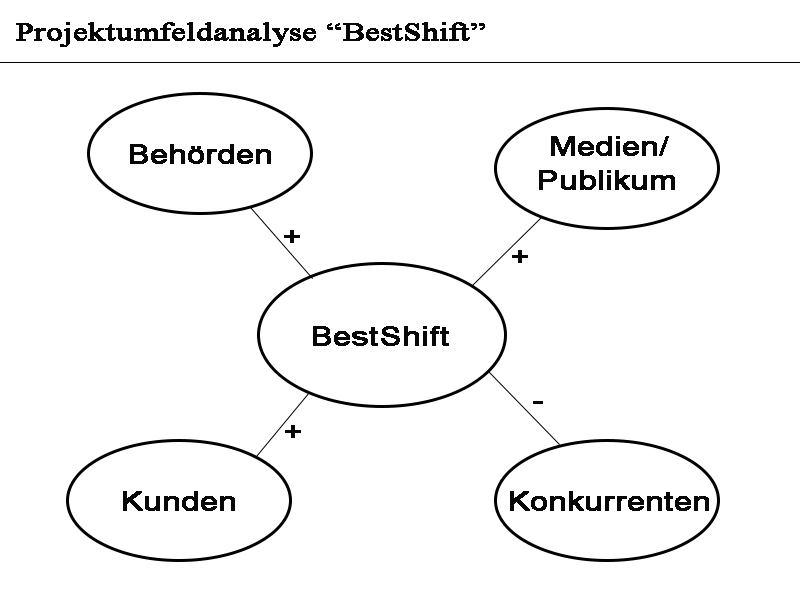
\includegraphics[scale=0.5]{images/Puma.jpg}

\newpage
\subsection{Kunden}
Das Produkt hat für Kunden einen kontinuierlich Erwerbsfähigen Nutzen durch die App,
denn je öfter die App benutzt wird um die Fahrweise des jeweiligen Kunden zu analysieren,
desto effizienter und Umweltschonender wird sie. 

\subsection{Medien/Publikum}
Von dem Publikum erwarten wir ebenfalls eine Positive Rückmeldung,
da der Umweltschonende Aspekt von BestShift eine positive Aura ausstrahlen lässt.

\subsection{Konkurrenten}
Einige Versuche hinsichtlich zur Datenanalyse via OBD-II gibt es schon am Markt,
allerdings finden diese keinen gemeinsamen Nenner mit BestShift.
Im Projekt BestShift wird nicht nur die Smartphone-App geliefert, die zur graphischen Darstellung der momentanen Fahrt dient, sondern auch eine Web-Applikation welche es erlaubt die erstellten Graphiken Retrospektiv zu betrachten.
Ebenfalls entwickeln wir unseren eigenen Car-PC, welches uns ebenfalls unabhängiger macht.
Deshalb definieren wir jeden möglichen Konkurrenten als negatives Umfeld.


\subsection{Behörden}
Die App könnte in gewissen Fällen ein revolutionäres Tool für Fahrschulen sein.
Da der Informationsfluss auf das Verständnis des Fahrschülers basiert, 
können hier Kommunikationsfehler entstehen. Das Entwickeln des Umweltschonenden Fahrgefühls ist
ebenfalls keine leichte angelegenheit, da es jahrelange Übung und Sammeln von Erfahrungen benötigt. Durch BestShift sind graphische Fahrverläufe betrachtbar, wodurch Verständnisfehler vermieden werden können. Aus diesem Grund sehen wir die Behörde als einen wahrscheinlich positiven Rückmelder.


\section{Ressourcenverwaltung}

\subsection{Software (App)}
Als Entwicklungsumgebung der Software werden Eclipse für Java und PyCharm für Python,
welche beide kostenlos Verfügbar sind und keine Lizenzen benötigen benutzt.

\subsection{Hardware}
Als Car PC wird ein Raspberry Pi 2 Modell B mit einem Gy521 Board und einem DHT22 Sensor verwendet. Mit dieser zusammenstellung wird der Preis gering gehalten und genaue Ergebnisse gemessen.

\subsection{Cloud}
Während der Fahrt werden die gesammelten Daten im CarPC gespeichert.
Nach der Fahrt allerdings, soll die Option geboten werden, die gesammelten Daten
in die Cloud zu transferieren. Dadurch ist eine sekundäre Sicherungsmethode der Daten
gegeben.